\documentclass{article}


\usepackage{arxiv}

\usepackage[utf8]{inputenc} % allow utf-8 input
\usepackage[T1]{fontenc}    % use 8-bit T1 fonts
\usepackage{hyperref}       % hyperlinks
\usepackage{url}            % simple URL typesetting
\usepackage{booktabs}       % professional-quality tables
\usepackage{amsfonts}       % blackboard math symbols
\usepackage{nicefrac}       % compact symbols for 1/2, etc.
\usepackage{microtype}      % microtypography
\usepackage{lipsum}
\usepackage{graphicx}
\usepackage{float}

\title{ECI2019 - Competencia Despegar \\ Clasificador de imágenes de hoteles}


\author{
  Leticia L. Rodríguez
}

\begin{document}
\maketitle

\begin{abstract}
En el presente informe se detalla el proceso llevado a cabo para a elaboración de un clasificador de imágenes de Hoteles en el contexto de las Competencias de Datos de la ECI 2019. 
\end{abstract}


% keywords can be removed
\keywords{Clasificación de Imágenes \and Tranfer Learning \and Redes Convolucionales \and Optimización de Redes Neuronales}

\section{Sobre Pytorch}

Pytorch sobre Tensorflow fue el framework elegido para la implementación. A diferencia de Keras, Pytorch provee mayor performance y mayor flexibilidad para implementar optimizaciones para el entramiento. 

La elección de Pytorch también se vio influída por su simple sintaxis y la facilidad para cargar y pre-procesar las imágenes.

\section{Preparación de los datos}

El pre-procesamiento de datos se vió relacionado con el framework elegido, Pytorch.

\subsection{Organización del filesystem}

Pytorch provee una forma simple de leer las imágenes desde el disco con sus correspondientes categorías utilizando la clase ImageFolder. 

Para que pueda asignar las categorias a cada imagen, precisa que los datos estén organizados de forma que cada categoria tenga una carpeta y dentro las imágenes correspondientes. 

Así que la primer tarea fue descargar las imágenes de testeo y entrenamiento, y organizarlas de forma que puedan ser leidas fácilmente con por el framework con su correspondiente categoria. Dado que las categorias o labels se encontraban en un csv, se usaron scripts de python que organicen los archivos como se indica en la figura \ref{directories}

\begin{figure}
  \begin{center}
    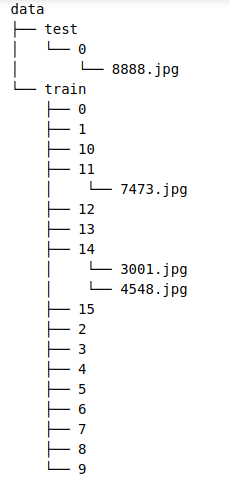
\includegraphics[width=120px]{img/directories.png}
    \caption{Organización de las imágenes en directorios para ser leidos por Pytorch}
    \label{directories}
  \end{center}
\end{figure}

 

\subsection{Construcción de los conjuntos de entrenamiento, validación y testeo}

En la competencia se proveen de sets de entrenamiento y testeo. Decidí reservar una porción de los datos de entrenamiento como validación de forma que sirvan para observar el progreso del entrenamiento y sobre todo condiciones como Overfitting (Sobreajuste). El 20\% de los datos seleccionados de manera aletoria del conjunto de entrenamiento fue usado como validación.

\subsection{Data Augmentation o Image Augmentation}

Por último, Pytorch permite construir un DataLoader que va a contener las imágenes pre-procesadas con transformaciones que indiquemos. En el caso del dataset de entrenamiento, podemos especificar transformaciones que agreguen Image Augmentation, es decir, que apliquen transformaciones como rotaciones, flipeos, redimensionamientos, crops, etc para darle variabilidad a los datos. 

En Pytorch, estas tranformaciones se aplican en las épocas sin agrandar el dataset pero generando diferencias en una misma imagen entre las épocas lo que permite que se puedan reajustar los pesos acorde a las diferentes variaciones. 

Hay varias tranformaciones disponibles provistas por Pytorch e incluso se pueden codear propias. En particular, trabajé con el siguiente pipeline de transformaciones:

\begin{figure}[H]
  \begin{center}
    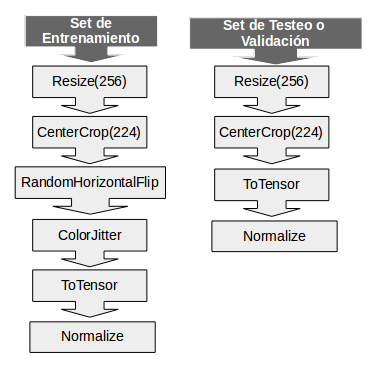
\includegraphics[width=250px]{img/transformaciones.png}lety
    \caption{ Pipeline de transformaciones aplicadas a los conjuntos de datos }
    \label{conn}
  \end{center}
\end{figure}


Justificación: 

\begin{itemize}
  \item Resize(256) $\rightarrow$ CenterCrop(224): Dado que el modelo va a usar Transfer Learning sobre modelos entrenados con tamaños de entrada 224x224x3, las imagenes son redimensionadas a 256x256x3 para luego, mediante CenterCrop, ignorar los bordes quedándo con el centro, donde podría estar la información más relevante. 
  \item ToTensor: Transforma los bits en un tensor
  \item Normalize: Normaliza los datos para mejorar convergencia  
\end{itemize}

Para el dataset de entrenamiento, además se incluyeron las siguientes transformaciones:

\begin{itemize}
  \item RandomHorizontalFlip: Debido al tipo de problema, una habitación vista de derecha a izquierda, o de izquierda a derecha pertenece a una misma categoría. Por ejemplo, una silla apuntando hacia la izquierda o la derecha no cambia la detección y poder invertir las imagenes permite darle mayor información al clasificador. 
  \item ColorJitter: Aplica cambios aletorios al brillo, constranste y saturación de la imagen. La idea es despegar un poco de los colores que se ven en la habitación. 
\end{itemize}

Otras transformaciones consideradas y descartadas: 

\begin{itemize}
  \item Grayscale: se probó convertir grayscale sin grandes resultados aparentemente porque los modelos pre-entrados usados trabajan con entradas a color. 
  \item RandomRotation: Dado que las habitaciones parten de un piso, rotarlas carece de sentido. Se probó con una pequeña rotación de 10 grados sin grandes cambios.
\end{itemize}

\subsection{Etiquetas y desbalanceo del conjunto de entrenamiento}

El conjunto de entrenamiento suministrado está desbalanceado, es decir, algunas categorías tienen demasiadas imágenes en comparación a otras. 

No modifiqué los datos ni excluí imágenes por esto. Simplemente, calculé los diferentes pesos de las categorías de las siguiente forma para ser usados por la función de pérdida (que va a ser un weighted categorical crossentropy, más información en las siguientes secciones).
 

\section{Modelado}
\label{sec:headings}

\subsection{Transferencia del aprendizaje - Transfer Learning}

En lugar de construir un modelo desde el llano, se optó por reentrenar un modelo existente y entrenado sobre el dataset Imagenet.

Se elige este enforque porque estos modelos se encuentran hiper optimizados y entrenados durante días sobre los datos. Lograr algo similar requeriría mucho tiempo y esfuerzo que carecería de sentido en este contexto. 

Igualmente, estos modelos son siempre un buen benchmark para evaluar cualquier modelo que se quiera diseñar desde cero. 

\begin{figure}
  \begin{center}
    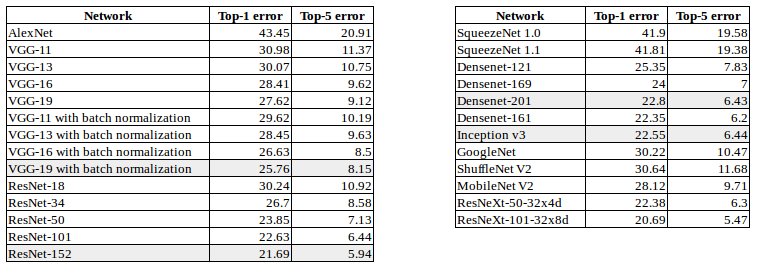
\includegraphics[width=450px]{img/pytorch-benchmark.png}
    \caption{Modelos pre-entrenados - Benchmark - Fuente: Pytorch}
    \label{models_bench}
  \end{center}
\end{figure}

Para la competencia, se probaron modelos simples de pocas capas, intermedios y con muchas capas. Se probó con VGG19 con BatchNormalization, Resnet18, AlexNet, Resnet50 y Resnet101. Sin embargo, aquellos que tienen más capas son los que mejores resultados tuvieron: \textbf{Resnet152} y \textbf{Denset201}. 

Adicionalmente, se probó el modelo inception que utiliza entradas de 299x299x3. Los resultados no fueron superiores que los dos detallados anteriormente.

La elección del modelo final tuvo 2 etapas. La primera relacionada con evaluar distintos modelos con diferentes learning rates, optimizadores y parámetors, y una segunda etapa, focalizada en la optimización de los modelos de interés.

De la primer etapa, se obtuvo el learning rate que hace que mejor decaiga la curva de funciones de pérdida (loss functions), optimizadores a utilizar, batch sizes a utilizar, 
 
En un comienzo, no todos los entrenamientos fueron bajo las mismas condiciones, hasta que se encontraron parámetros y modelos interesantes que fueron expuestos a fine tuning que detallo en la próxima sección.

Los resultados acompañan la lógica de que modelos más profundos captan mejor los detalles de los datos pero tienden a overfittear y ese fue el principal problema que apareció durante el entrenamiento. Además, la elección de Resnet152 y Densenet201 como candidatos está también justificada por los benchmarks presentados en la figura \ref{models_bench}.

Por falta de tiempo, excluyo de la optimización a VGG19 con Batch Normalization e Inception, que me parecen bastante interesantes y que me hubiera gustado profundizar. 

\subsubsection{Bottleneck features vs. entrenamiento del modelo completo}

También se consideró usar los modelos como features extractors, es decir, usar los pesos sobre los datos de entrenamiento y entrenar un modelo más pequeño que utilize esta información de entrada. Pero los resultados no fueron tan buenos como reentrenar el modelo completo.\\

La técnica de reentrenar el modelo consiste en usar los pesos pre-calculados como pesos iniciales y reentrenar el modelo completo, no únicamente las capas finales. Este segundo aproach tuvo resultados superiores.


\begin{figure}[H]
  \begin{center}
    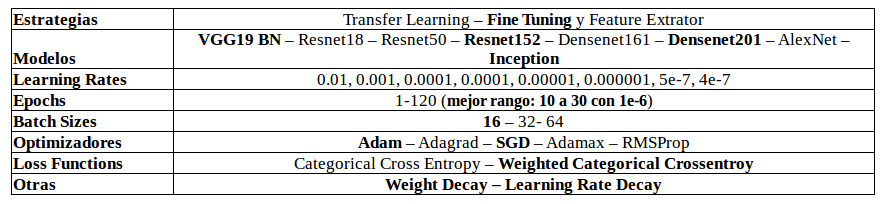
\includegraphics[width=450px]{img/tested.png}
    \caption{Combinaciones y modelos testeados. En negrita, las combinaciones que tuvieron mejores resultados}
    \label{models_bench}
  \end{center}
\end{figure}

\subsection{El modelo}

El modelo que mejor funcionó fue un Resnet152. Las redes neuronales residuales proponen una solución al desvanecimiento del gradiente durante el entrenamiento. Esta compuesta por bloques residuales que poseen ademas un enlace que lleva al final del bloque aplicando la función identidad sobre la entrada. Figura \ref{conn} 

\begin{figure}[H]
  \begin{center}
    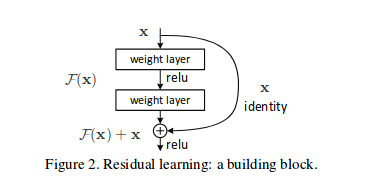
\includegraphics[width=200px]{img/resnet_connection.png}
    \caption{Bloque Resnet}
    \label{conn}
  \end{center}
\end{figure}

La última capa de esta red la he reemplazado por una capa completamente conectada que retorna 16 salidas, cada una correspondiente a la probabilidad de cada categoría. 

\begin{figure}[H]
  \begin{center}
    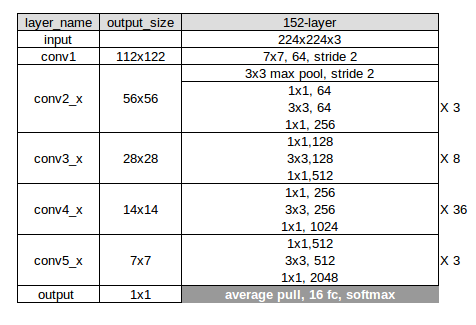
\includegraphics[width=250px]{img/network.png}
    \caption{Resnet-152 modificada . Salida 16 nodos. }
    \label{conn}
  \end{center}
\end{figure}


\section{Evaluación de los Resultados}
\label{sec:others}
% \cite{kour2014real,kour2014fast} and see \cite{hadash2018estimate}.



% \bibliographystyle{unsrt}  
% %\bibliography{references}  %%% Remove comment to use the external .bib file (using bibtex).
% %%% and comment out the ``thebibliography'' section.
% %%% Comment out this section when you \bibliography{references} is enabled.
% \begin{thebibliography}{1}
%
% \bibitem{kour2014real}
% George Kour and Raid Saabne.
% \newblock Real-time segmentation of on-line handwritten arabic script.
% \newblock In {\em Frontiers in Handwriting Recognition (ICFHR), 2014 14th
%   International Conference on}, pages 417--422. IEEE, 2014.
%
% \bibitem{kour2014fast}
% George Kour and Raid Saabne.
% \newblock Fast classification of handwritten on-line arabic characters.
% \newblock In {\em Soft Computing and Pattern Recognition (SoCPaR), 2014 6th
%   International Conference of}, pages 312--318. IEEE, 2014.
%
% \bibitem{hadash2018estimate}
% Guy Hadash, Einat Kermany, Boaz Carmeli, Ofer Lavi, George Kour, and Alon
%   Jacovi.
% \newblock Estimate and replace: A novel approach to integrating deep neural
%   networks with existing applications.
% \newblock {\em arXiv preprint arXiv:1804.09028}, 2018.
%
% \end{thebibliography}
%

\end{document}
